%!TeX root = thesis-main.tex
\begin{figure}[!ht]
  %%% PROBLEM 1: thr %%% 
  \begin{subfigure}[b]{0.32\textwidth}
    \centering
    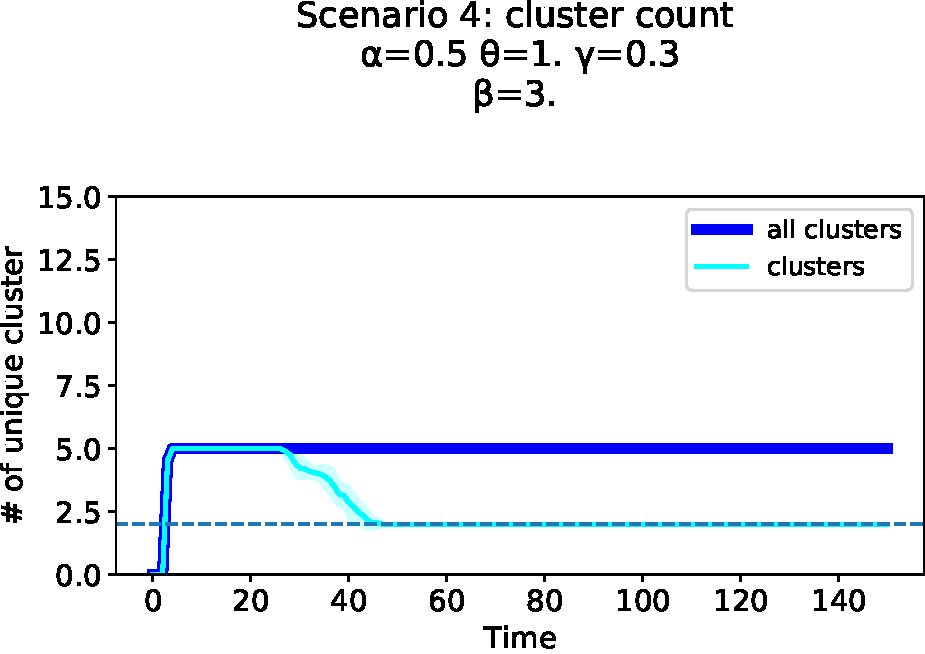
\includegraphics[width=\textwidth]{papers/swarm-intelligence2021/img/simulations/overlay_0_021_α-0.5_θ-1._γ-0.3_β-3._ω-0._ζ-0..pdf}
  \end{subfigure}
  \hfill
  \begin{subfigure}[b]{0.32\textwidth}
    \centering
    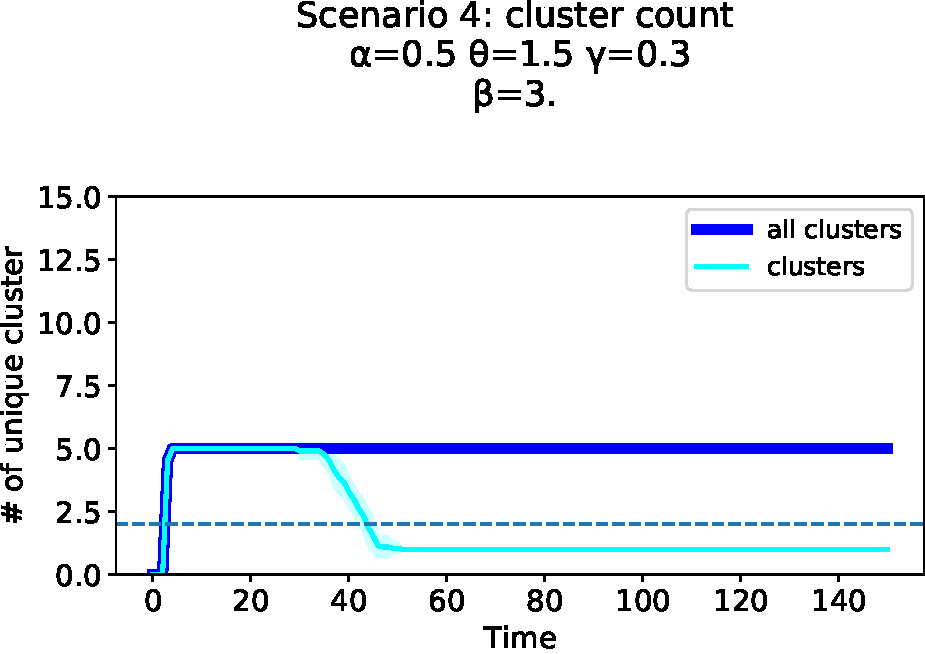
\includegraphics[width=\textwidth]{papers/swarm-intelligence2021/img/simulations/overlay_0_021_α-0.5_θ-1.5_γ-0.3_β-3._ω-0._ζ-0..pdf}
  \end{subfigure}
  \hfill
  \begin{subfigure}[b]{0.32\textwidth}
    \centering
    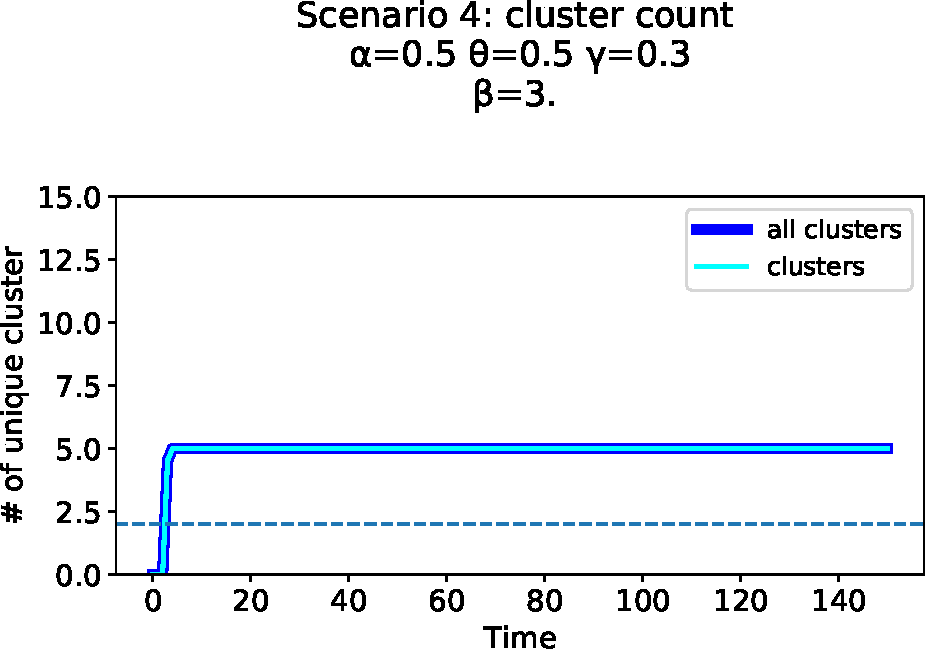
\includegraphics[width=\textwidth]{papers/swarm-intelligence2021/img/simulations/overlay_0_021_α-0.5_θ-0.5_γ-0.3_β-3._ω-0._ζ-0..pdf}
  \end{subfigure}
  %%% PROBLEM 2: density %%% 
  \begin{subfigure}[b]{0.32\textwidth}
    \centering
    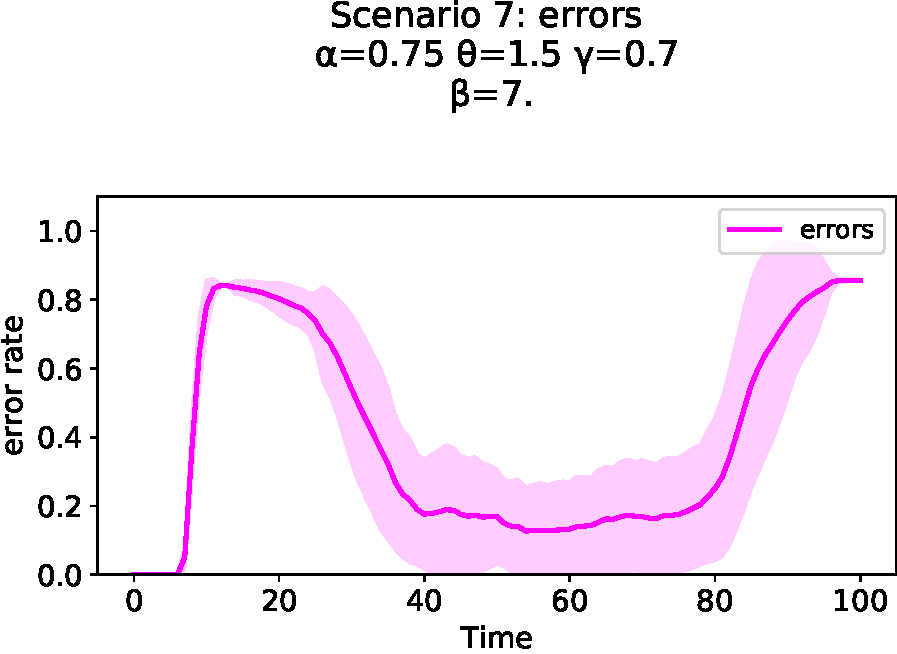
\includegraphics[width=\textwidth]{papers/swarm-intelligence2021/img/simulations/standard-updatable-errors_0_08_α-0.75_θ-0.5_γ-0.1_β-5._ω-0._ζ-0..pdf}
  \end{subfigure}
  \hfill
  \begin{subfigure}[b]{0.32\textwidth}
    \centering
    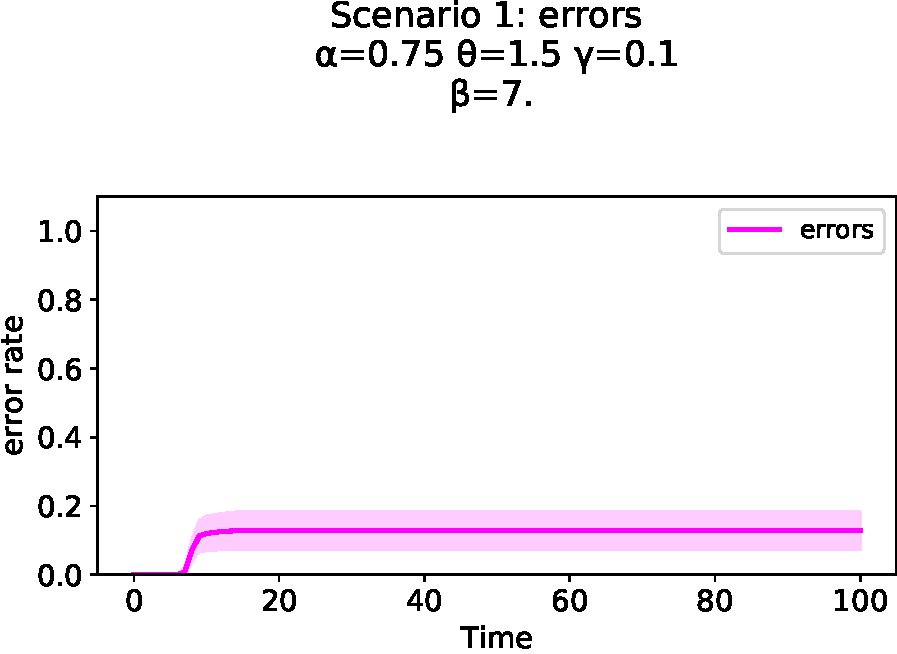
\includegraphics[width=\textwidth]{papers/swarm-intelligence2021/img/simulations/standard-errors_0_08_α-0.75_θ-1.5_γ-0.1_β-7._ω-0._ζ-0..pdf}
  \end{subfigure}
  \hfill
  \begin{subfigure}[b]{0.32\textwidth}
    \centering
    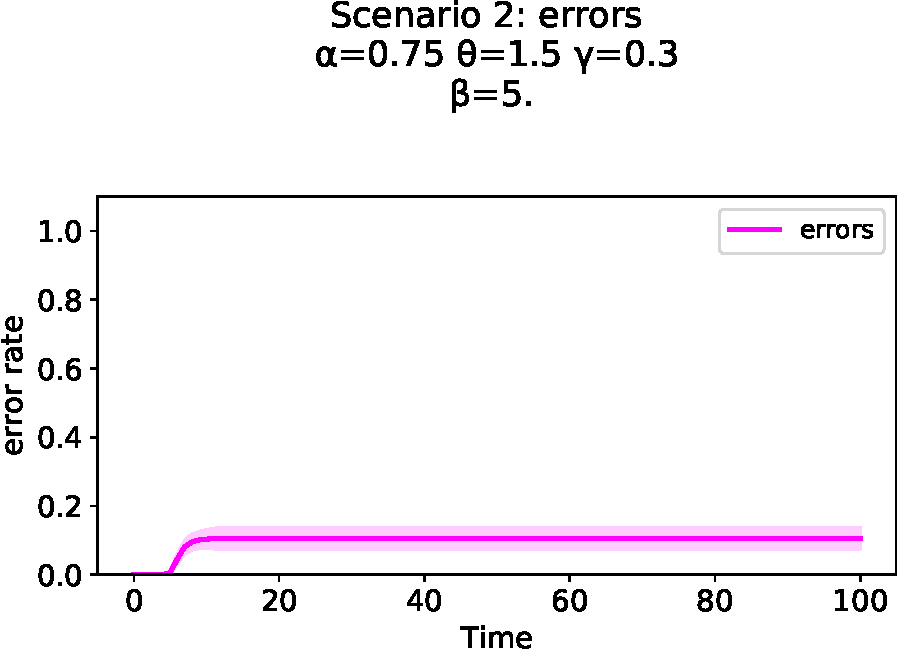
\includegraphics[width=\textwidth]{papers/swarm-intelligence2021/img/simulations/stretched-errors_0_08_α-0.75_θ-1.5_γ-0.3_β-5._ω-0._ζ-0..pdf}
  \end{subfigure}
  \\
  %% Focus 3: mobility
  \begin{subfigure}[b]{0.32\textwidth}
    \centering
    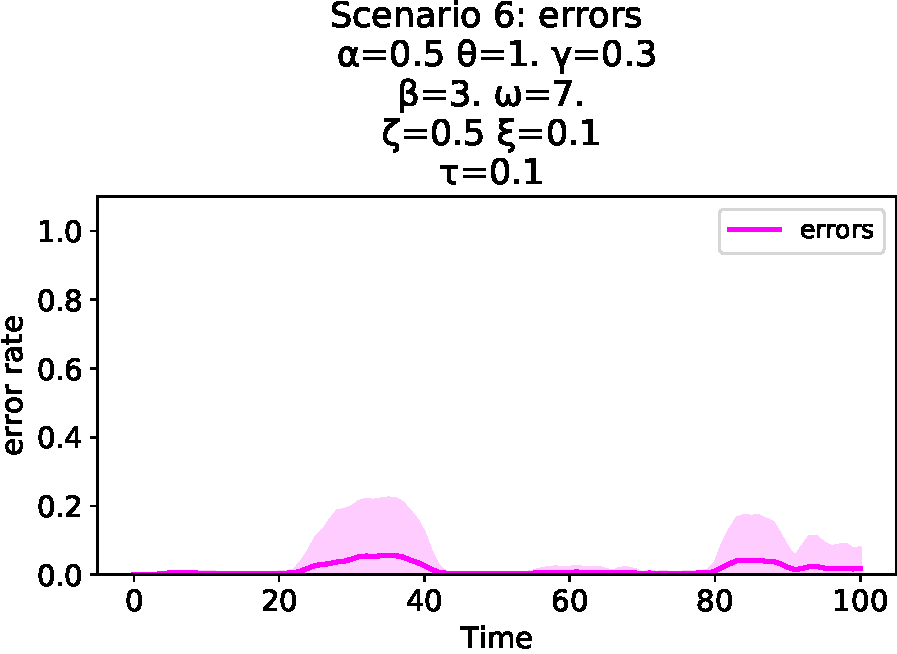
\includegraphics[width=\textwidth]{papers/swarm-intelligence2021/img/simulations/movement-errors_0_08_α-0.5_θ-1._γ-0.3_β-3._ω-7._ζ-0.5.pdf}
  \end{subfigure}
  \hfill
  \begin{subfigure}[b]{0.32\textwidth}
    \centering
    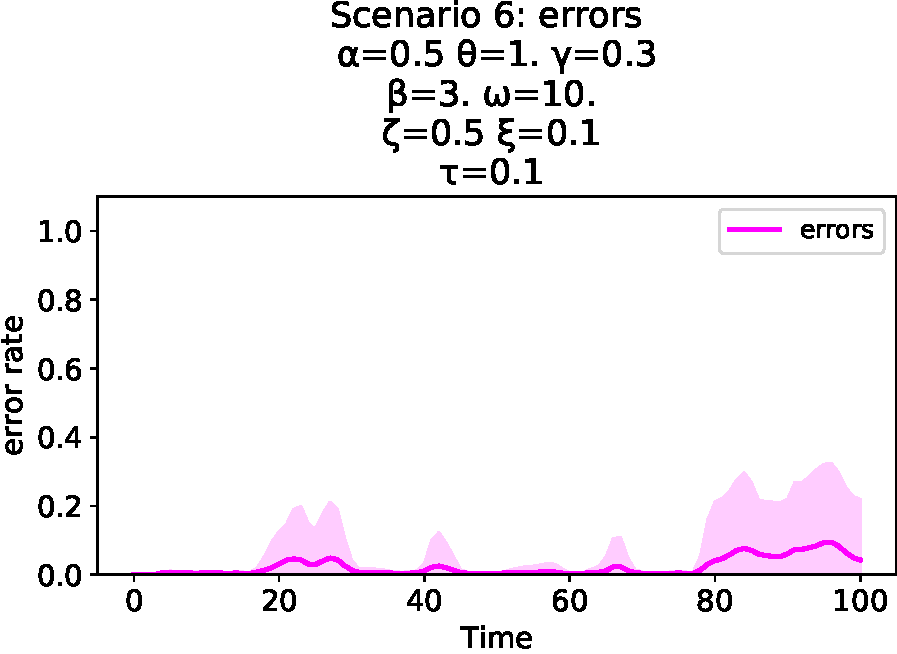
\includegraphics[width=\textwidth]{papers/swarm-intelligence2021/img/simulations/movement-errors_0_08_α-0.5_θ-1._γ-0.3_β-3._ω-10._ζ-0.5.pdf}
  \end{subfigure}
  \hfill
  \begin{subfigure}[b]{0.32\textwidth}
    \centering
    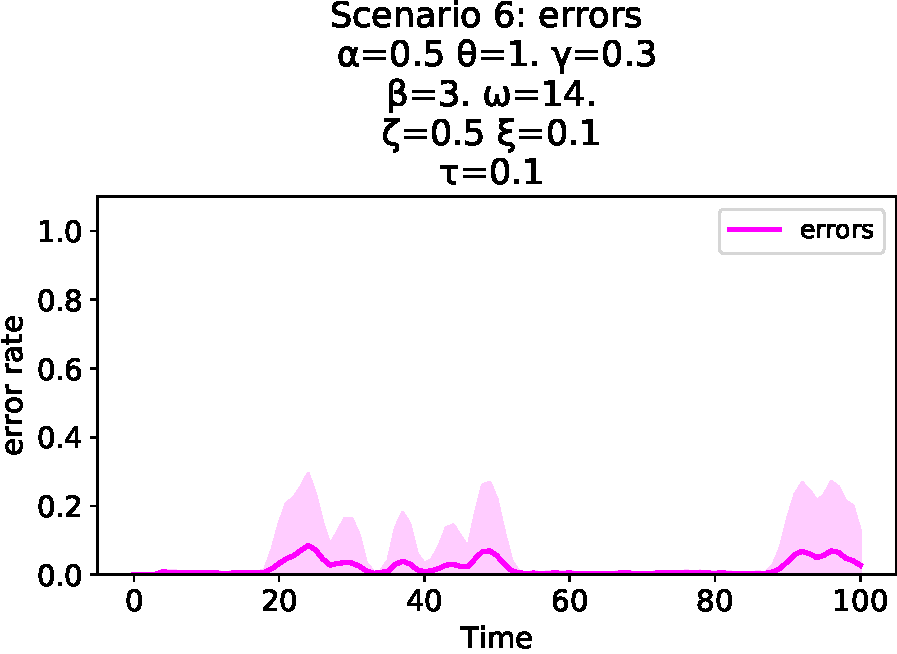
\includegraphics[width=\textwidth]{papers/swarm-intelligence2021/img/simulations/movement-errors_0_08_α-0.5_θ-1._γ-0.3_β-3._ω-14._ζ-0.5.pdf}
  \end{subfigure}
  \\
  %% Focus 4: movement range
  \begin{subfigure}[b]{0.32\textwidth}
    \centering
    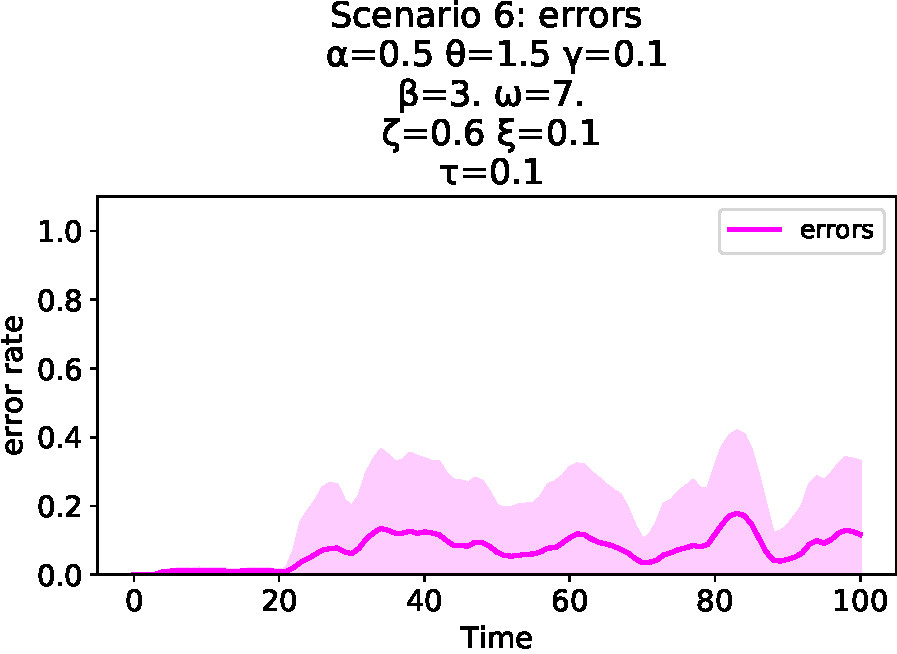
\includegraphics[width=\textwidth]{papers/swarm-intelligence2021/img/simulations/movement-errors_0_08_α-0.5_θ-1.5_γ-0.1_β-3._ω-7._ζ-0.6.pdf}
  \end{subfigure}
  \hfill
  \begin{subfigure}[b]{0.32\textwidth}
    \centering
    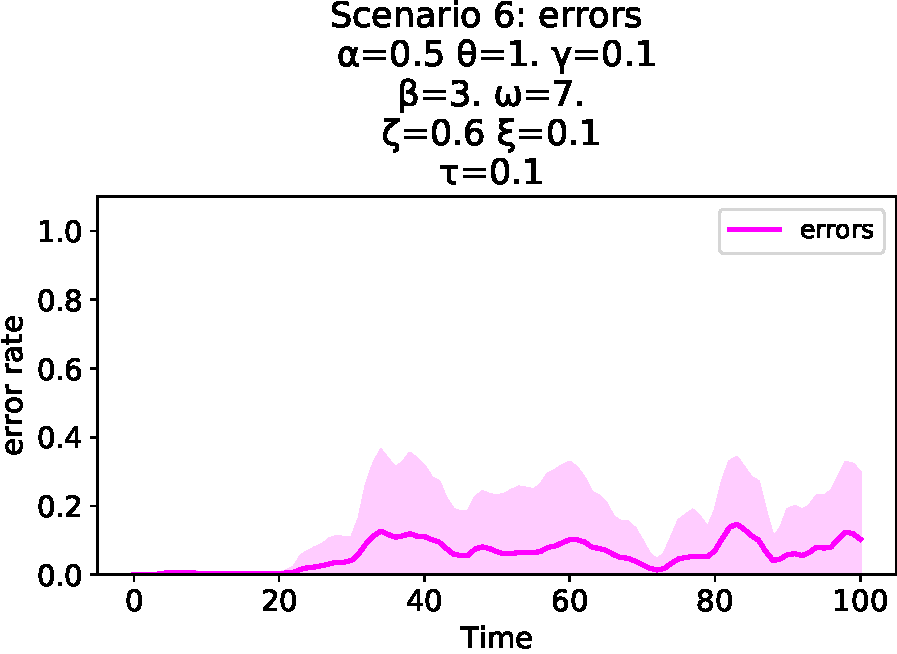
\includegraphics[width=\textwidth]{papers/swarm-intelligence2021/img/simulations/movement-errors_0_08_α-0.5_θ-1._γ-0.1_β-3._ω-7._ζ-0.6.pdf}
  \end{subfigure}
  \hfill
  \begin{subfigure}[b]{0.32\textwidth}
    \centering
    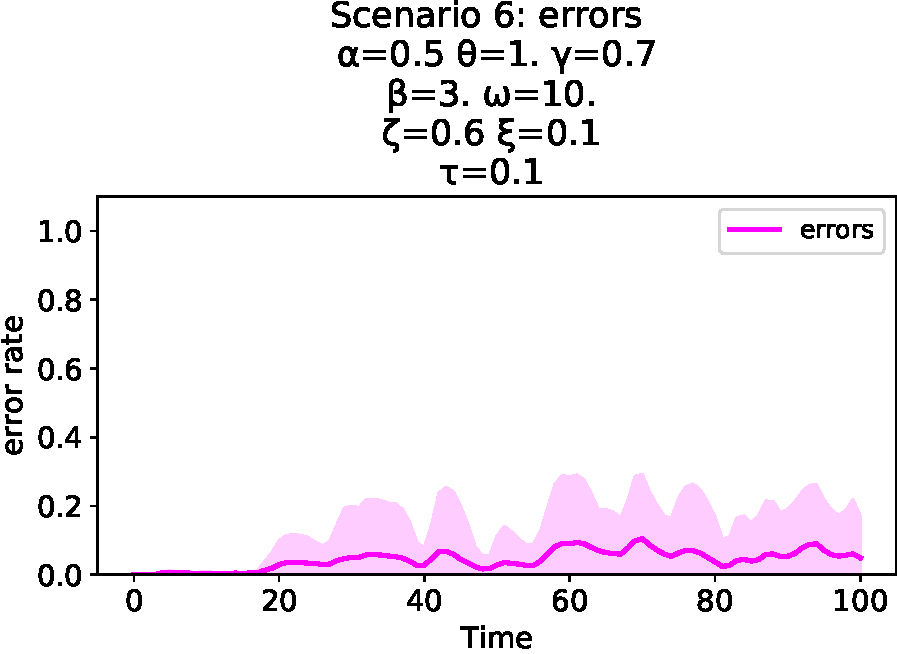
\includegraphics[width=\textwidth]{papers/swarm-intelligence2021/img/simulations/movement-errors_0_08_α-0.5_θ-1._γ-0.7_β-3._ω-10._ζ-0.6.pdf}
  \end{subfigure}
  %% Focus 4: movement range
  \begin{subfigure}[b]{0.32\textwidth}
    \centering
    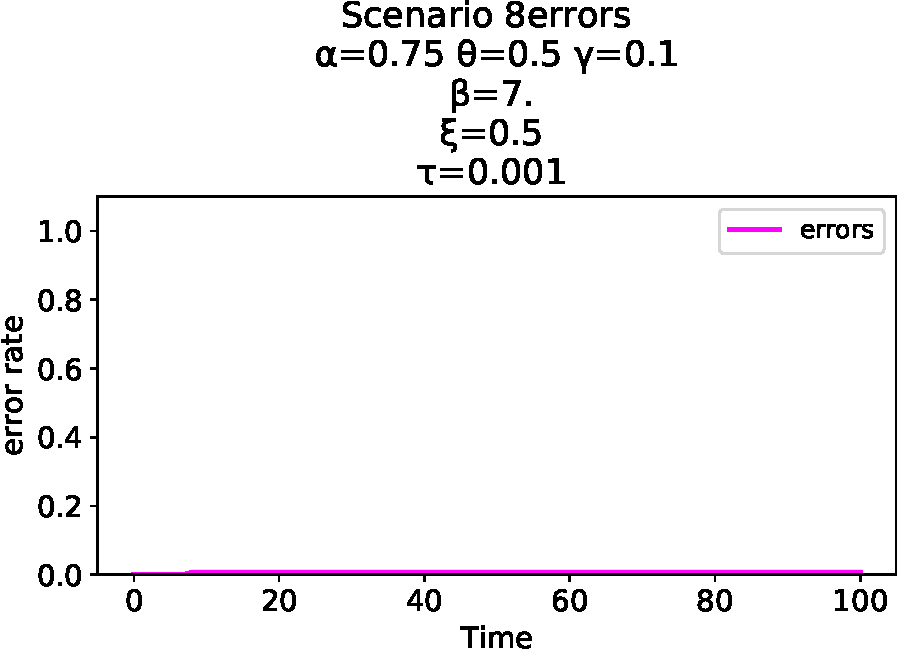
\includegraphics[width=\textwidth]{papers/swarm-intelligence2021/img/simulations/failScenario_0_08_α-0.75_θ-0.5_γ-0.1_β-7._ω-0._ζ-0._ξ-0.5_τ-0.001}
  \end{subfigure}
  \hfill
  \begin{subfigure}[b]{0.32\textwidth}
    \centering
    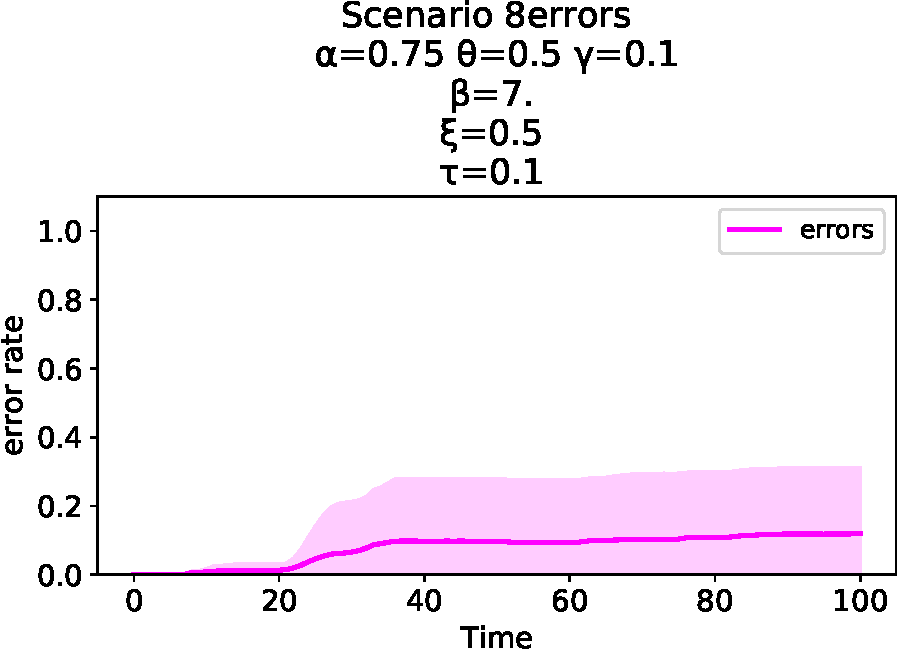
\includegraphics[width=\textwidth]{papers/swarm-intelligence2021/img/simulations/failScenario_0_08_α-0.75_θ-0.5_γ-0.1_β-7._ω-0._ζ-0._ξ-0.5_τ-0.1}
  \end{subfigure}
  \hfill
  \begin{subfigure}[b]{0.32\textwidth}
    \centering
    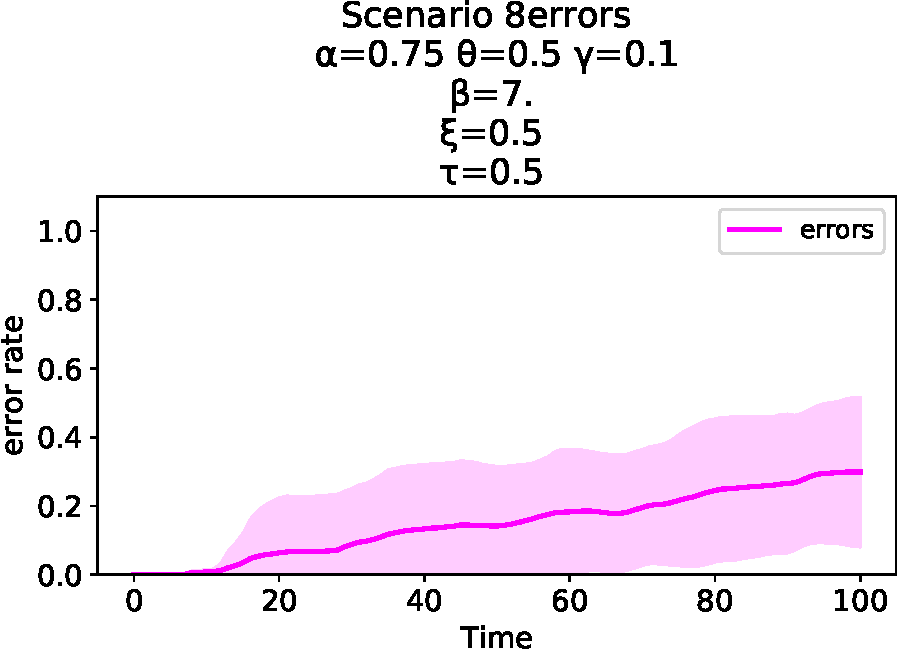
\includegraphics[width=\textwidth]{papers/swarm-intelligence2021/img/simulations/failScenario_0_08_α-0.75_θ-0.5_γ-0.1_β-7._ω-0._ζ-0._ξ-0.5_τ-0.5}
  \end{subfigure}
  \caption[Main examples of bad clustering results]{Main examples of bad clustering results.
  In the first line, the images show different behaviour varying $\theta$.
  In the second line, the plots show how the algorithm does not handle well low-density robot swarms.
  In the third line, the charts show how the algorithm handles various movement speeds.
  The fourth line shows how the exploration range impacts the clustering results.
  \rev{Finally, the last line shows how failures impact performance.}
  }
  \label{fig:bad-simulation-results}
\end{figure}